\documentclass[12pt,]{article}
\usepackage[left=1in,top=1in,right=1in,bottom=1in]{geometry}
\newcommand*{\authorfont}{\fontfamily{phv}\selectfont}
\usepackage{lmodern}


  \usepackage[T1]{fontenc}
  \usepackage[utf8]{inputenc}



\usepackage{abstract}
\renewcommand{\abstractname}{}    % clear the title
\renewcommand{\absnamepos}{empty} % originally center

\renewenvironment{abstract}
 {{%
    \setlength{\leftmargin}{0mm}
    \setlength{\rightmargin}{\leftmargin}%
  }%
  \relax}
 {\endlist}

\makeatletter
\def\@maketitle{%
  \newpage
%  \null
%  \vskip 2em%
%  \begin{center}%
  \let \footnote \thanks
    {\fontsize{18}{20}\selectfont\raggedright  \setlength{\parindent}{0pt} \@title \par}%
}
%\fi
\makeatother




\setcounter{secnumdepth}{0}

\usepackage{longtable,booktabs}

\usepackage{graphicx,grffile}
\makeatletter
\def\maxwidth{\ifdim\Gin@nat@width>\linewidth\linewidth\else\Gin@nat@width\fi}
\def\maxheight{\ifdim\Gin@nat@height>\textheight\textheight\else\Gin@nat@height\fi}
\makeatother
% Scale images if necessary, so that they will not overflow the page
% margins by default, and it is still possible to overwrite the defaults
% using explicit options in \includegraphics[width, height, ...]{}
\setkeys{Gin}{width=\maxwidth,height=\maxheight,keepaspectratio}

\title{Education and Library Patronage  }



\author{\Large Rudd Fawcett\vspace{0.05in} \newline\normalsize\emph{Phillips Academy}  }


\date{}

\usepackage{titlesec}

\titleformat*{\section}{\normalsize\bfseries}
\titleformat*{\subsection}{\normalsize\itshape}
\titleformat*{\subsubsection}{\normalsize\itshape}
\titleformat*{\paragraph}{\normalsize\itshape}
\titleformat*{\subparagraph}{\normalsize\itshape}





\newtheorem{hypothesis}{Hypothesis}
\usepackage{setspace}

\makeatletter
\@ifpackageloaded{hyperref}{}{%
\ifxetex
  \PassOptionsToPackage{hyphens}{url}\usepackage[setpagesize=false, % page size defined by xetex
              unicode=false, % unicode breaks when used with xetex
              xetex]{hyperref}
\else
  \PassOptionsToPackage{hyphens}{url}\usepackage[unicode=true]{hyperref}
\fi
}

\@ifpackageloaded{color}{
    \PassOptionsToPackage{usenames,dvipsnames}{color}
}{%
    \usepackage[usenames,dvipsnames]{color}
}
\makeatother
\hypersetup{breaklinks=true,
            bookmarks=true,
            pdfauthor={Rudd Fawcett (Phillips Academy)},
             pdfkeywords = {},  
            pdftitle={Education and Library Patronage},
            colorlinks=true,
            citecolor=black,
            urlcolor=black,
            linkcolor=black,
            pdfborder={0 0 0}}
\urlstyle{same}  % don't use monospace font for urls

% set default figure placement to htbp
\makeatletter
\def\fps@figure{htbp}
\makeatother

\usepackage{fontspec}
\setmainfont{Times New Roman}
\setlength\parindent{2em}
\setlength\parskip{0em}
\usepackage{indentfirst}
\usepackage[bottom]{footmisc}
\usepackage{etoolbox}
\AtBeginEnvironment{quote}{\singlespacing\small}
\usepackage{caption}
\captionsetup[table]{labelformat=empty}


% add tightlist ----------
\providecommand{\tightlist}{%
\setlength{\itemsep}{0pt}\setlength{\parskip}{0pt}}

\begin{document}
	
% \pagenumbering{arabic}% resets `page` counter to 1 
%
% \maketitle

{% \usefont{T1}{pnc}{m}{n}
\setlength{\parindent}{0pt}
\thispagestyle{plain}
{\fontsize{18}{20}\selectfont\raggedright 
\maketitle  % title \par  

}

{
   \vskip 13.5pt\relax \normalsize\fontsize{11}{12} 
\textbf{\authorfont Rudd Fawcett} \hskip 15pt \emph{\small Phillips Academy}   

}

}








\begin{abstract}

    \hbox{\vrule height .2pt width 39.14pc}

    \vskip 8.5pt % \small 

\noindent This study examines the association between a state's degree of
education, quantified by the public high school graduation rate, and the
users of public libraries on a per 100,000 person basis to attempt to
answer the question: are smarter states using libraries more?


    \hbox{\vrule height .2pt width 39.14pc}


\end{abstract}


\vskip 6.5pt


\noindent \doublespacing \newpage

\section{Introduction}\label{introduction}

Reading makes you smarter. You've heard it from your parents and
teachers, and their claim is well documented. Though intelligence or
``smarts'' may be relatively unquantifiable measures, reading is a
proven intellectual exercise that expands your vocabulary and capacity
for analytical thinking, for example.\footnote{Cunningham, Anne, and
  Keith Stanovich. 2001. \emph{What Reading Does For The Mind}. Ebook.
  Journal of Direct Instruction.
  \url{http://www.csun.edu/~krowlands/Content/Academic_Resources/Reading/Useful}
  Articles/Cunningham-What Reading Does for the Mind.pdf.} For many
Americans, however, books are a commodity item, nonessential in
comparison to food and other basics. Thankfully, the United States is
home to the fifth largest public library system in the world, according
to a recent study of global data and statistics compiled by the Online
Computer Library (OCLC).\footnote{``Global Library Statistics''. 2017.
  \emph{Oclc.Org}.
  \url{https://www.oclc.org/en/global-library-statistics.html}.} With
over 9,000 total libraries --- almost three libraries for every 100,000
citizens as of 2012 --- ``libraries are a quintessential part of how
Americans learn and engage with their local communities.''\footnote{``A
  History Of US Public Libraries · DPLA Omeka''. 2017. \emph{Dp.La.}
  \url{https://dp.la/exhibitions/exhibits/show/history-us-public-libraries}.}

With such access to books and knowledge, it would seem that there is a
correlation between a quantifiable measure of intelligence or academic
achievement --- public high school graduation rates --- and the users of
public libraries per 100,000 people. So, do smarter people use libraries
more? Examining individual states and regions across America, this study
aims to answer that question using data from the National Center for
Education Statistics (NCES) and the Institute of Museum and Library
Services (IMLS) from the 2014 fiscal year.

\newpage

\section{Variables and Definitions}\label{variables-and-definitions}

Throughout this study, two variables will primarily examined: NCES
reported graduation rate of public high schools by state and IMLS
reported users of public libraries by state. It is important that both
of these variables measure publically accessible institutions, as there
is thus a determination that all citizens could be included in both
pools. Additionally, the total number of public libraries adjusted by
state population will be reported on a per 100,00 people per state and
region, to be known as ``Libraries.''

NCES public high school graduation rates are measured as an Adjusted
Cohort Graduation Rate (ACGR), which tracks transfers and those who
graduate within four years with a high school diploma. The NCES defines
such graduation rate as, simply: ``the percentage of public high school
students who graduate on time.'' These rates will serve as a
quantifiable measurement of education by state. Public high school
graduation rates by state will hence be known as ``Graduation Rates.''

Library ``users'' from IMLS data have been adjusted per state
population, and are reported on a per 100,000 person per state basis
using population data included in the same IMLS report. The IMLS defines
``users'' --- to hence be down as ``Library Users'' --- as follows:

\begin{quote}
``A registered user is a library user who has applied for and received
an identification number or card from the public library that has
established conditions under which the user may borrow library materials
or gain access to other library resources. Note: Files should have been
purged within the past three (3) years.''\footnote{``State Profiles: FY
  2014 Public Libraries Survey (Data) \textbar{} Data Catalog''. 2017.
  \emph{Data.Imls.Gov}.
  \url{https://data.imls.gov/Public-Libraries-Survey/State-Profiles-FY-2014-Public-Libraries-Survey-Dat/mph3-8hz6}}
\end{quote}

For the purposes of this study, graduation rates will serve as the
explanatory variable and library users as a response variable. This
decision will serve the driving question of: ``are smarter people using
libraries more?'' As previously mentioned, all data is per the 2014
fiscal year.

\newpage

\section{Analysis}\label{analysis}

Before examining the relationship between Library Users and Graduation
Rates, it is important to first contextualize and analyze the
distribution of Libraries and Library Users across America.
\vspace{20pt}

\begin{figure}[htbp]
\centering
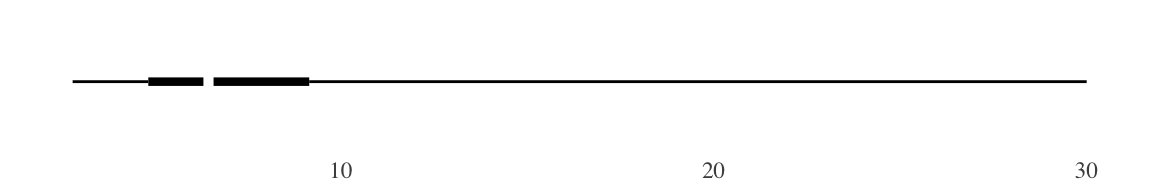
\includegraphics{report_files/figure-latex/unnamed-chunk-2-1.pdf}
\caption{Distribution of Librariesacross America.}
\end{figure}

\begin{longtable}[]{@{}rrrrrr@{}}
\toprule
Min. & 1st Qu. & Median & Mean & 3rd Qu. & Max.\tabularnewline
\midrule
\endhead
2.8 & 4.83 & 6.44 & 8.12 & 9.14 & 30\tabularnewline
\bottomrule
\end{longtable}

\vspace{10pt}

As is apparent in Figure 1, there is a positive-skew distribution in the
data over the range from 2.797 Libraries to 30.002 Libraries. The
positive-skew can also be seen in the summary statistics for the
boxplot, as the mean is greater than the median. Given that the
interquartile range is relatively small in comparison to the range of
the entire data set, there is rather little variability in terms of the
overall distribution of Libraries. Six outlying states, such as Vermont
(30.002 Libraries) and Maine (20.375 Libraries), are responsible for
pulling the skew in the positive direction. On average, states have
8.037 Libraries as calculated in relation to the state's population.
\newpage
Unlike the distribution of Libraries, the data for Library Users is
approximately normal.

\vspace{20pt}

\begin{figure}[htbp]
\centering
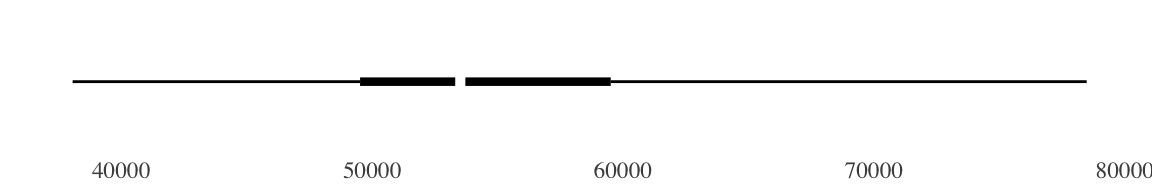
\includegraphics{report_files/figure-latex/unnamed-chunk-4-1.pdf}
\caption{Distribution of Library Users across America.}
\end{figure}

\begin{longtable}[]{@{}rrrrrr@{}}
\toprule
Min. & 1st Qu. & Median & Mean & 3rd Qu. & Max.\tabularnewline
\midrule
\endhead
38100 & 49500 & 53500 & 54400 & 59500 & 78500\tabularnewline
\bottomrule
\end{longtable}

\vspace{0pt}

Over the range from 38,053 to 78,466 Library Users, the distribution is
approximately understood due to the difference between the mean (53,507
Library Users) and median (54,413 Library Users). Ohio (78,466 Library
Users) and Minnesota (75,319 Library Users) are the only two outliers in
the dataset and lie in the positive direction. Vermont and Maine, which
have the most Libraries, are not outliers for the most Library Users.
Vermont (51,623 Library Users) and Maine (57,094 Library Users) fall
just below the median and just below the third quartile, respectively,
both within the interquartile range. \newpage
Just as Libraries and Library Users were examined, so must Graduation
Rates. A boxplot shows the large spread of data for Graduation Rates
across the country. As is evident visually in the boxplot, and
numerically because the median is greater than the mean, the data is
skewed in the negative direction.

\vspace{20pt}

\begin{figure}[htbp]
\centering
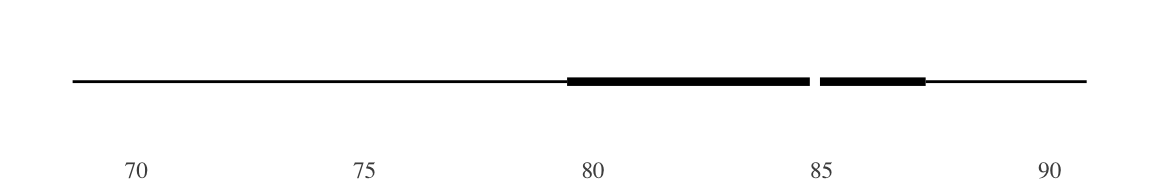
\includegraphics{report_files/figure-latex/unnamed-chunk-6-1.pdf}
\caption{Distribution of Graduation Rates across America.}
\end{figure}

\begin{longtable}[]{@{}rrrrrr@{}}
\toprule
Min. & 1st Qu. & Median & Mean & 3rd Qu. & Max.\tabularnewline
\midrule
\endhead
68.6 & 79.4 & 84.8 & 83.3 & 87.3 & 90.8\tabularnewline
\bottomrule
\end{longtable}

\vspace{0pt}

While a test for traditional outliers yields none, there are still three
relative outliers which pull the center of the graph in the negative
direction. These three states, New Mexico, Nevada, and Oregon have the
lowest Graduation Rates in America, with values of 68.6, 71.3, and 73.8
respectively. The large interquartile range suggests that there is not
that much variability in the data.

\newpage

\section{Further Analysis}\label{further-analysis}

Given the background context behind Library Users and Graduation Rates,
it is now possible to analyze a possible association between the two.
Plotting Graduation Rates as the explanatory variable and Library Users
as a response variable produces the following results on a scatterplot:

\vspace{20pt}

\begin{figure}[htbp]
\centering
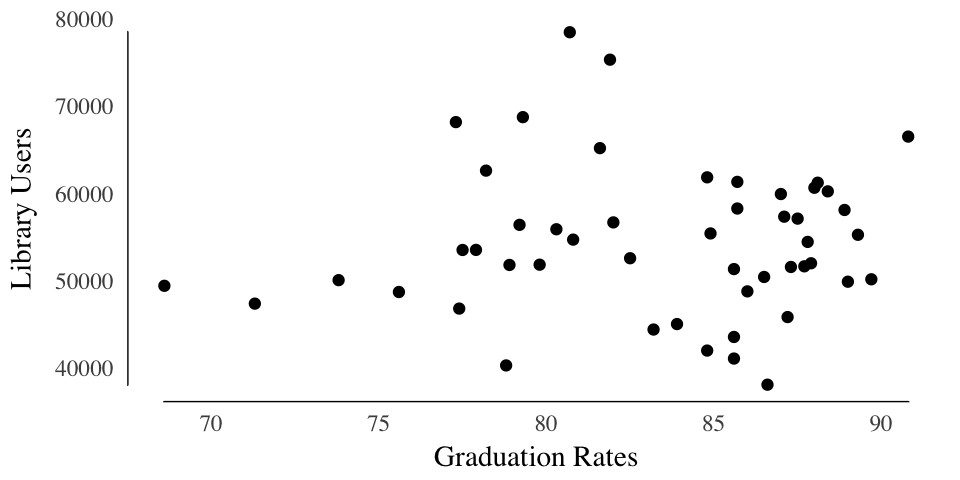
\includegraphics{report_files/figure-latex/unnamed-chunk-8-1.pdf}
\caption{The relationship between Graduation Rates and Library Users.}
\end{figure}

\vspace{0pt}

\newpage

The scatterplot depicted in Figure 4 shows a weak, nonlinear association
between Graduation Rates and Library Users. There do not appear to be
any outliers in the data that cannot be explained by either their
distribution in comparison to their explanatory or response variable
pools. Further investigating the relationship with a Least Squares
Regression Line results in the following:

\vspace{20pt}

\begin{figure}[htbp]
\centering
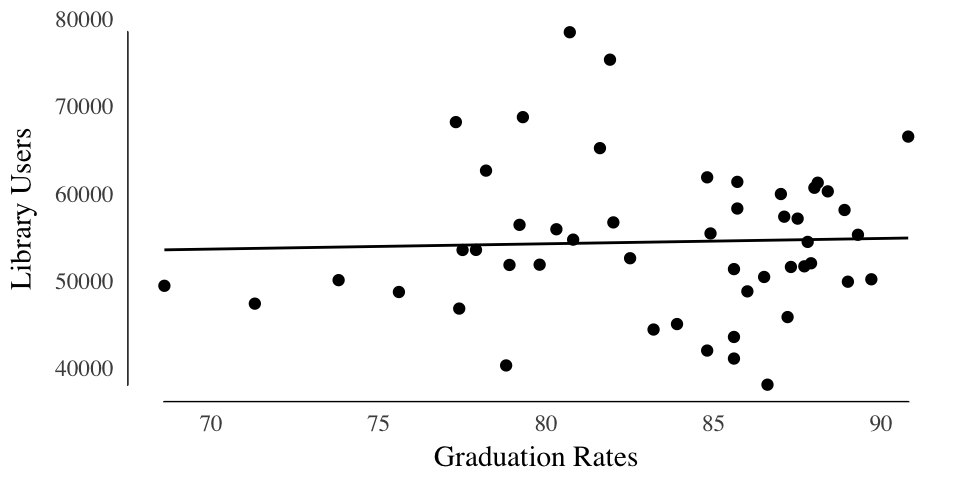
\includegraphics{report_files/figure-latex/unnamed-chunk-9-1.pdf}
\caption{The relationship between Graduation Rates and Library Users
with Least Squares Regression Line.}
\end{figure}

\begin{longtable}[]{@{}llll@{}}
\toprule
r & coeff. determination & slope & y-intercept\tabularnewline
\midrule
\endhead
0.0362 & 0.0013 & 82.1098 & 2.150758e-05\tabularnewline
\bottomrule
\end{longtable}

\vspace{0pt}

The correlation coefficient for the LSRL in Figure 5 is 0.036,
reaffirming that there is a very weak positive linear association
between Graduation Rates and Library Users. 0.0013\% of the variation in
Library Users can be explained by the approximate linear relationship
with Graduation Rate. For every percent increase in Graduation Rates,
the model predicts an almost negligable average increase of 82 Library
Users. At a Graduation Rates value of 0 people, the model predicts a
Library User value of 2.15078E-5 units. This value, as it stands, is
rather meaningless in the context of an extremely weak correlation
coefficient.

A residual plot of the association between Graduation Rates and Library
Users would suggest, however, that a the best type of regression model
is, in fact, linear.

\vspace{20pt}

\begin{figure}[htbp]
\centering
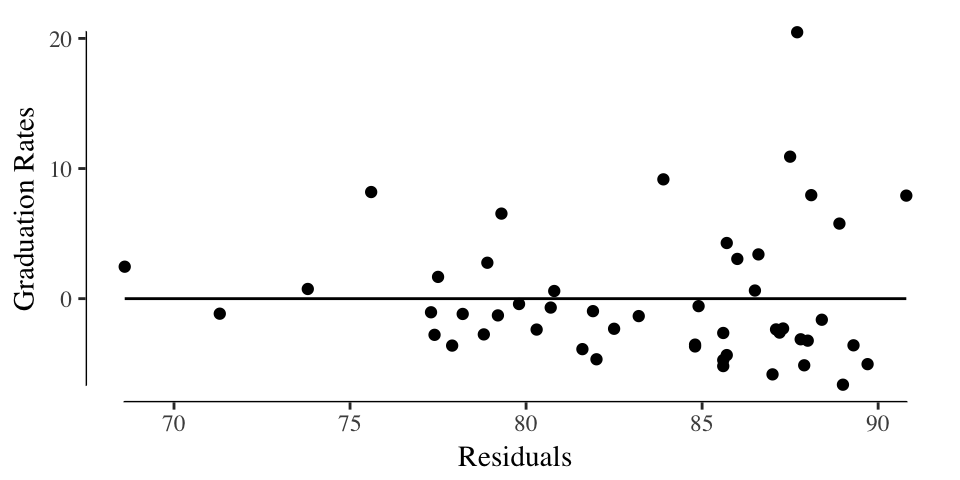
\includegraphics{report_files/figure-latex/unnamed-chunk-11-1.pdf}
\caption{A residual plot for Graduation Rates and Library Users data.}
\end{figure}

\vspace{0pt}

Figure 6 graphs the residuals of Graduation Rates and Library Users on
the y-axis and the Graduation Rates on the x-axis. The plot shows a
random pattern, with variation in the sign of the values. Such a pattern
would indicate that a linear model is appropriate for the data set,
though it does not comment on the fit of the LSRL. Had the residual plot
been non-random, with a parabolic shape, for example, it would indicate
that another type of regression analysis would better serve this
dataset.

\newpage

\section{Conclusion}\label{conclusion}

Throughout the statistical analysis and data exploration above, there is
no association between Graduation Rates and Library Users. As Graduation
Rates serve as a quantitative measure of educational attainment, and
there is no association between the data, it is not possible to answer
the project's framing question of ``do smarter people use libraries
more?''

\section{Further Study}\label{further-study}

This study neglects any hidden variables, and the effect that they may
have on Libraries, Graduation Rates, and Library Users. It would be
interesting to examine the effect of GDP per 100,000 people per state,
specifically looking at the association between GDP and Graduation Rate,
or GDP and Libraries.

Additionally, further research could be done by region in order to see
if there are trends in Graduation Rates or Library Users across America.
See the appendix for more graphs that begin to explore Graduation Rates
and Library Users by region.

\newpage

\begin{center}
\textbf{Bibliography}
\end{center}

\setstretch{1.0} \noindent
``A History Of US Public Libraries · DPLA Omeka''. 2017. \emph{Dp.La.}
\url{https://dp.la/exhibitions/exhibits/show/history-us-public-libraries}.
\newline
\newline
\noindent
Cunningham, Anne, and Keith Stanovich. 2001. \emph{What Reading Does For
The Mind}. Ebook. Journal of Direct Instruction.
\url{http://www.csun.edu/~krowlands/Content/Academic_Resources/Reading/Useful}
Articles/Cunningham-What Reading Does for the Mind.pdf. \newline
\newline
\noindent
``Global Library Statistics''. 2017. \emph{Oclc.Org}.
\url{https://www.oclc.org/en/global-library-statistics.html}. \newline
\newline
\noindent
``State Profiles: FY 2014 Public Libraries Survey (Data) \textbar{} Data
Catalog''. 2017. \emph{Data.Imls.Gov}.
\url{https://data.imls.gov/Public-Libraries-Survey/State-Profiles-FY-2014-Public-Libraries-Survey-Dat/mph3-8hz6}
\newline
\newline
\noindent
``The Condition Of Education - Elementary And Secondary Education -
Student Effort, Persistence And Progress - Public High School Graduation
Rates - Indicator April (2017)''. 2017. \emph{Nces.Ed.Gov.}
\url{https://nces.ed.gov/programs/coe/indicator_coi.asp}.

\newpage

\begin{center}
\textbf{Appendix}
\end{center}

\begin{table}[!h]

\caption{\label{tab:unnamed-chunk-12}Table 1: Compiled Dataset}
\centering
\resizebox{\linewidth}{!}{\begin{tabular}[t]{llrrrrrrr}
\toprule
\multicolumn{2}{c}{ } & \multicolumn{4}{c}{Raw Values} & \multicolumn{3}{c}{Adjusted per 100,000 people per state} \\
\cmidrule(l{2pt}r{2pt}){3-6} \cmidrule(l{2pt}r{2pt}){7-9}
State & Region & Population & Graduation Rate & Libraries & Users & Libraries per HundredK & Users per HundredK & Books per HundredK\\
\midrule
AK & West & 735601 & 75.6 & 102 & 358089 & 13.866213 & 48679.79 & 330918.0\\
AL & South & 4822023 & 89.3 & 311 & 2663716 & 6.449575 & 55240.63 & 195811.7\\
AR & South & 2915918 & 84.9 & 235 & 1615238 & 8.059211 & 55393.81 & 216205.6\\
AZ & West & 6667241 & 77.4 & 231 & 3118825 & 3.464701 & 46778.35 & 123437.1\\
CA & West & 38340074 & 82.0 & 1170 & 21723648 & 3.051637 & 56660.42 & 170603.3\\
\addlinespace
CO & West & 5264890 & 77.3 & 272 & 3588616 & 5.166300 & 68161.27 & 195952.9\\
CT & Northeast & 3596080 & 87.2 & 243 & 1647190 & 6.757358 & 45805.15 & 405375.6\\
DE & South & 925244 & 85.6 & 34 & 379791 & 3.674706 & 41047.66 & 177544.0\\
FL & South & 19839251 & 77.9 & 555 & 10615421 & 2.797485 & 53507.17 & 159295.3\\
GA & South & 10344907 & 78.8 & 408 & 4164735 & 3.943970 & 40258.80 & 160496.0\\
\addlinespace
HI & West & 1404054 & 81.6 & 52 & 915100 & 3.703561 & 65175.56 & 235969.1\\
IA & Midwest & 3092341 & 90.8 & 570 & 2056436 & 18.432637 & 66500.95 & 388060.6\\
ID & West & 1634465 & 78.9 & 155 & 846363 & 9.483225 & 51782.27 & 264533.4\\
IL & Midwest & 12880580 & 85.6 & 801 & 5606184 & 6.218664 & 43524.31 & 337747.0\\
IN & Midwest & 6483802 & 87.1 & 452 & 3716275 & 6.971218 & 57316.29 & 375846.8\\
\addlinespace
KS & Midwest & 2893957 & 85.7 & 381 & 1774222 & 13.165365 & 61307.82 & 321379.0\\
KY & South & 4395295 & 88.0 & 281 & 2664920 & 6.393200 & 60631.20 & 205512.2\\
LA & South & 4629284 & 77.5 & 368 & 2476596 & 7.949394 & 53498.47 & 256970.5\\
MA & Northeast & 6587339 & 87.3 & 468 & 3395801 & 7.104538 & 51550.42 & 474918.1\\
MD & South & 5828289 & 87.0 & 203 & 3491938 & 3.483012 & 59913.60 & 218519.7\\
\addlinespace
ME & Northeast & 1330089 & 87.5 & 271 & 759409 & 20.374576 & 57094.60 & 474497.9\\
MI & Midwest & 9898193 & 79.8 & 653 & 5128464 & 6.597164 & 51812.12 & 329004.1\\
MN & Midwest & 5417838 & 81.9 & 364 & 4080678 & 6.718547 & 75319.31 & 269711.3\\
MO & Midwest & 6044917 & 87.8 & 389 & 3289934 & 6.435159 & 54424.80 & 277843.8\\
MS & South & 2994079 & 80.8 & 237 & 1637307 & 7.915623 & 54684.83 & 188422.7\\
\addlinespace
MT & West & 988533 & 86.0 & 119 & 481933 & 12.038040 & 48752.34 & 259586.2\\
NC & South & 9861952 & 85.6 & 408 & 5059879 & 4.137112 & 51307.07 & 169862.2\\
ND & Midwest & 739482 & 86.6 & 93 & 281392 & 12.576371 & 38052.58 & 311504.5\\
NE & Midwest & 1868969 & 88.9 & 293 & 1085590 & 15.677093 & 58084.97 & 316523.9\\
NH & Northeast & 1323259 & 88.1 & 233 & 809993 & 17.608042 & 61211.98 & 442904.1\\
\addlinespace
NJ & Northeast & 8791894 & 89.7 & 451 & 4408002 & 5.129725 & 50137.11 & 321069.6\\
NM & West & 2085287 & 68.6 & 123 & 1029945 & 5.898469 & 49391.04 & 206652.4\\
NV & West & 2795962 & 71.3 & 88 & 1323756 & 3.147396 & 47345.28 & 153719.4\\
NY & Northeast & 19378102 & 79.2 & 1072 & 10925440 & 5.532018 & 56380.34 & 365439.6\\
OH & Midwest & 11525088 & 80.7 & 762 & 9043300 & 6.611663 & 78466.21 & 371209.7\\
\addlinespace
OK & South & 3888566 & 82.5 & 216 & 2043524 & 5.554747 & 52552.12 & 183927.2\\
OR & West & 3919020 & 73.8 & 229 & 1961047 & 5.843298 & 50039.22 & 251922.7\\
PA & Northeast & 12702379 & 84.8 & 644 & 5330482 & 5.069916 & 41964.44 & 202955.8\\
RI & Northeast & 1051511 & 83.2 & 71 & 466618 & 6.752188 & 44375.95 & 402572.1\\
SC & South & 4652360 & 80.3 & 223 & 2599480 & 4.793266 & 55874.44 & 195744.0\\
\addlinespace
SD & Midwest & 852175 & 83.9 & 149 & 383507 & 17.484672 & 45003.32 & 329417.5\\
TN & South & 6469352 & 87.9 & 289 & 3362436 & 4.467217 & 51974.85 & 181800.5\\
TX & South & 26448193 & 89.0 & 880 & 13187230 & 3.327259 & 49860.61 & 152802.9\\
UT & West & 2900872 & 84.8 & 143 & 1793578 & 4.929552 & 61828.93 & 229019.3\\
VA & South & 8326289 & 85.7 & 379 & 4850306 & 4.551848 & 58252.91 & 210653.1\\
\addlinespace
VT & Northeast & 626630 & 87.7 & 188 & 323486 & 30.001755 & 51623.13 & 469196.5\\
WA & West & 6968170 & 78.2 & 371 & 4361927 & 5.324210 & 62597.88 & 192728.7\\
WI & Midwest & 5732981 & 88.4 & 466 & 3452345 & 8.128407 & 60219.02 & 327872.4\\
WV & South & 1852994 & 86.5 & 181 & 933968 & 9.767976 & 50403.19 & 271686.3\\
WY & West & 582658 & 79.3 & 78 & 400460 & 13.386927 & 68729.86 & 428548.5\\
\bottomrule
\end{tabular}}
\end{table}

\noindent
\textit{Sources: IMLS FY 2014 Public Libraries Survey, NCES FY 2014 Public High School Graduation Rates.}

\newpage

\vspace{20pt}

\begin{figure}[htbp]
\centering
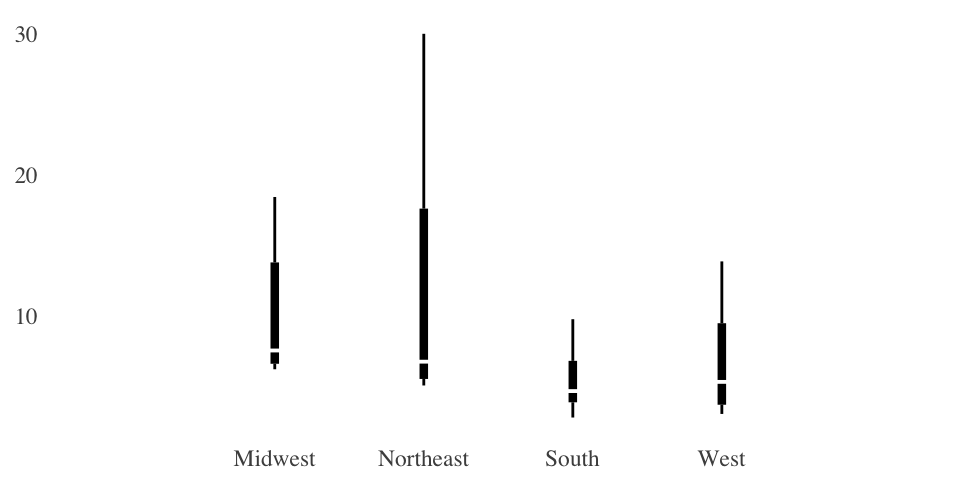
\includegraphics{report_files/figure-latex/unnamed-chunk-13-1.pdf}
\caption{Library count by region.}
\end{figure}

\vspace{0pt}

\vspace{20pt}

\begin{figure}[htbp]
\centering
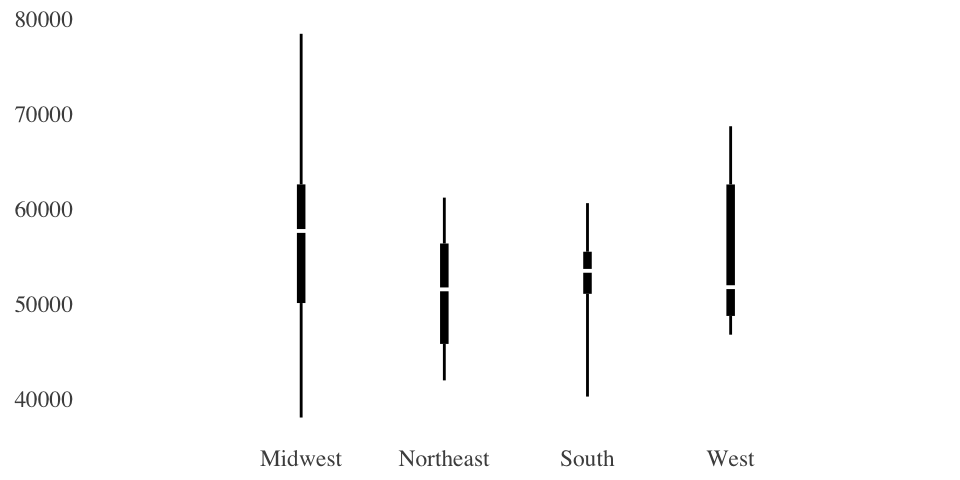
\includegraphics{report_files/figure-latex/unnamed-chunk-14-1.pdf}
\caption{Library Users by region.}
\end{figure}

\vspace{0pt}

\vspace{20pt}

\begin{figure}[htbp]
\centering
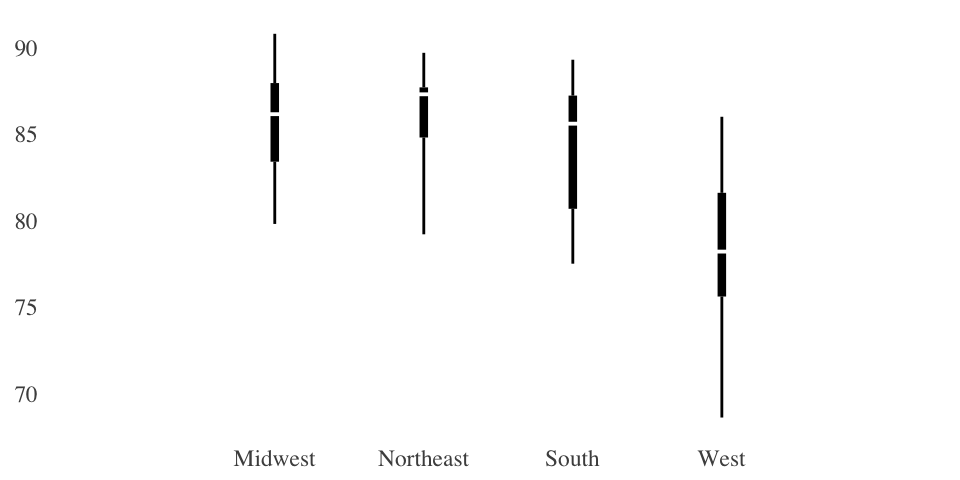
\includegraphics{report_files/figure-latex/unnamed-chunk-15-1.pdf}
\caption{Graduation Rates by region.}
\end{figure}

\vspace{0pt}

\vspace{20pt}

\begin{figure}[htbp]
\centering
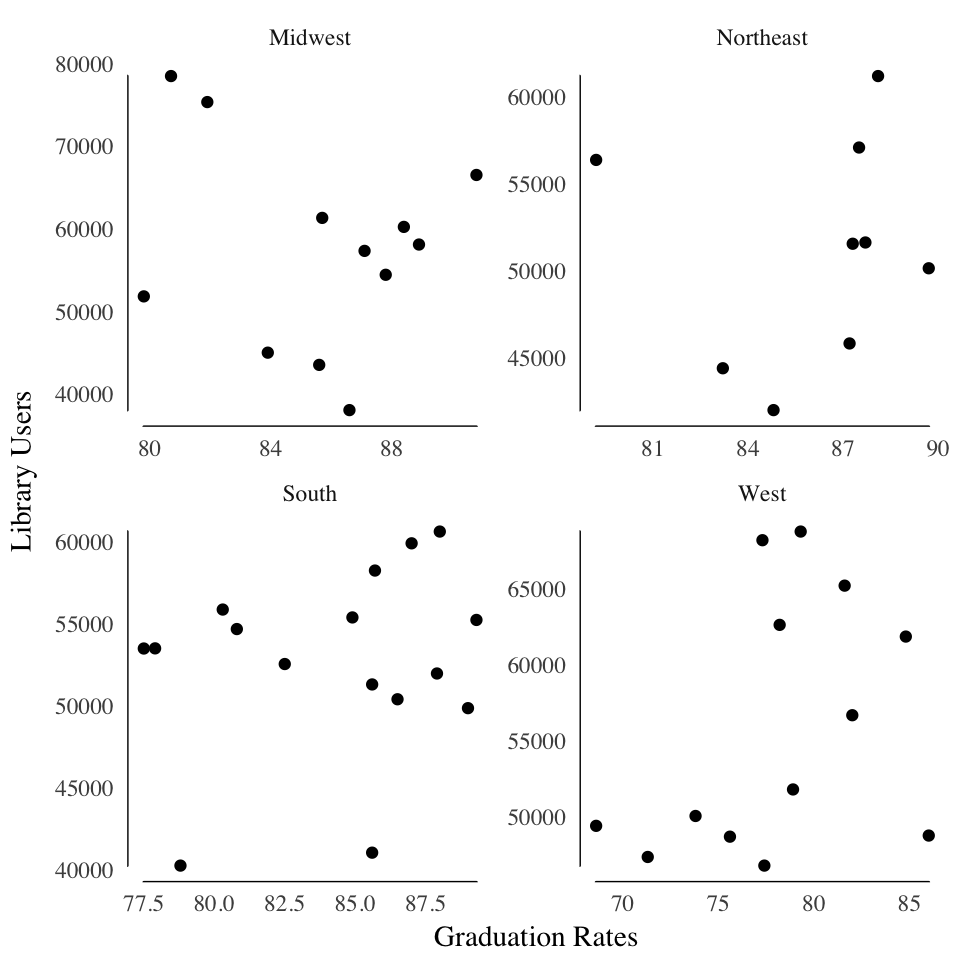
\includegraphics{report_files/figure-latex/unnamed-chunk-16-1.pdf}
\caption{Association between Graduation Rates and Library Users data by
region.}
\end{figure}

\vspace{0pt}




\newpage
\singlespacing 
\end{document}
